\chapter{TINJAUAN PUSTAKA}
\label{chap:tinjauanpustaka}

\section{Hasil Penelitian Terdahulu}
\label{sec:hasil_terdahulu}

Penelitian mengenai peningkatan kemampuan navigasi robot bergerak otonom telah berke\-mbang pesat dalam beberapa tahun terakhir, terutama melalui pemanfaatan berbagai jenis sensor dan metode pengambilan keputusan adaptif. Integrasi sensor digunakan untuk meningkat\-kan kualitas persepsi lingkungan, sedangkan metode kecerdasan komputasional diterapkan untuk menghasilkan perilaku navigasi yang lebih aman dan responsif terhadap perubahan kondisi lingkungan. Beberapa penelitian terdahulu yang memiliki keterkaitan dengan topik penelitian ini digunakan sebagai dasar dalam merancang sistem yang diusulkan.

Choi dan Kim (\cite{Choi2023}) mengembangkan sistem fusi sensor yang menggabungkan kamera inframerah termal dan LiDAR untuk meningkatkan kemampuan deteksi objek pada kendaraan otonom. Penelitian tersebut memanfaatkan data dari kedua sensor sebagai masukan bagi model deteksi berbasis pembelajaran mendalam sehingga objek dapat dikenali dengan lebih baik dibandingkan penggunaan sensor tunggal. Hasil penelitian menunjukkan bahwa integrasi kamera termal dan LiDAR mampu meningkatkan kualitas persepsi lingkungan, khususnya pada kondisi yang menantang bagi sensor visual konvensional. Meskipun demikian, penelitian tersebut difokuskan pada deteksi objek dan tidak membahas pemanfaatan informasi termal untuk mendukung navigasi robot maupun mengatasi keterbatasan \textit{blind-spot} pada LiDAR dua dimensi.

Haider et al. (\cite{Haider2022}) mengusulkan sistem navigasi robot bergerak berbasis sensor fusion dan \textit{adaptive neuro-fuzzy inference system} untuk meningkatkan kemampuan penghindaran obstacle pada lingkungan yang padat. Sistem yang dikembangkan mampu men\-yesuaikan perilaku navigasi berdasarkan kondisi lingkungan yang diamati sensor sehingga me\-nghasilkan pergerakan yang lebih aman dan stabil dibandingkan pendekatan konvensional. Hasil pengujian menunjukkan bahwa penerapan mekanisme fuzzy adaptif memberikan peningkatan performa navigasi pada lingkungan yang kompleks. Namun demikian, penelitian tersebut tidak memanfaatkan kamera termal sebagai sumber informasi tambahan dan tidak membahas permasalahan obstacle yang berada pada area \textit{blind-spot} LiDAR.

Berdasarkan kedua penelitian tersebut, dapat dilihat bahwa integrasi sensor LiDAR dan kamera termal memiliki potensi untuk meningkatkan kualitas persepsi lingkungan, sedangkan pendekatan fuzzy adaptif mampu meningkatkan kualitas pengambilan keputusan pada sistem navigasi robot. Akan tetapi, penelitian yang secara khusus menggabungkan kedua pendekatan tersebut untuk mengatasi keterbatasan deteksi obstacle pada area \textit{blind-spot} LiDAR masih relatif terbatas.

Oleh karena itu, penelitian ini mengusulkan sistem navigasi robot beroda otonom berbasis logika fuzzy dengan fusi sensor LiDAR dan kamera termal. Berbeda dengan penelitian sebelumnya, kamera termal tidak hanya digunakan sebagai sensor deteksi tambahan, tetapi dimanfaatkan untuk membentuk informasi traversability termal dan \textit{virtual LaserScan} yang kemudian digabungkan dengan traversability berbasis LiDAR. Informasi hasil fusi tersebut selanjutnya digunakan oleh pengendali fuzzy Mamdani untuk mengatur parameter \textit{Artificial Potential Field} secara adaptif berdasarkan kondisi lingkungan yang diamati. Dengan demikian, penelitian ini tidak hanya berfokus pada peningkatan persepsi lingkungan, tetapi juga pada peningkatan keselamatan navigasi melalui kemampuan deteksi obstacle berprofil rendah dan pengambilan keputusan yang lebih adaptif.

\begin{table}[H]
\centering
\scriptsize
\caption{Perbandingan penelitian terdahulu dengan penelitian yang diusulkan.}
\label{tab:penelitian_terdahulu}
\renewcommand{\arraystretch}{1.0}
\setlength{\tabcolsep}{3pt}

\begin{tabularx}{0.95\textwidth}{|>{\raggedright\arraybackslash}p{2.1cm}|X|X|X|}
\hline
\textbf{Aspek} &
\textbf{Choi dan Kim (2023)} &
\textbf{Haider et al. (2022)} &
\textbf{Penelitian Ini} \\
\hline

Tujuan penelitian &
Meningkatkan kemampuan deteksi objek menggunakan fusi LiDAR dan kamera termal pada kendaraan otonom &
Meningkatkan kemampuan navigasi robot menggunakan sensor fusion dan pengendali neuro-fuzzy adaptif &
Meningkatkan keselamatan navigasi robot melalui fusi LiDAR dan kamera termal serta pengendali fuzzy adaptif \\
\hline

Sensor utama &
LiDAR dan kamera termal &
LiDAR dan sensor jarak untuk navigasi robot &
LiDAR 2D dan kamera termal \\
\hline

Fokus pemrosesan &
Deteksi objek berbasis pembelajaran mendalam &
Navigasi dan penghindaran obstacle &
Navigasi, estimasi traversability, dan penghindaran obstacle \\
\hline

Penanganan blind-spot LiDAR &
Tidak dibahas &
Tidak dibahas &
Menggunakan informasi termal untuk mendeteksi obstacle pada area blind-spot LiDAR \\
\hline

Representasi lingkungan &
Objek hasil deteksi &
Data sensor fusion untuk navigasi &
Traversability LiDAR, traversability termal, dan traversability efektif hasil fusi sensor \\
\hline

Pemanfaatan kamera termal &
Sebagai sumber informasi untuk deteksi objek &
Tidak digunakan &
Sebagai sumber informasi traversability dan pembentukan \textit{virtual LaserScan} \\
\hline

Metode pengambilan keputusan &
Klasifikasi berbasis \textit{deep learning} &
Adaptive Neuro-Fuzzy Inference System (ANFIS) &
Logika fuzzy Mamdani \\
\hline

Metode navigasi &
Tidak membahas navigasi &
Navigasi berbasis sensor fusion dan neuro-fuzzy &
Navigasi berbasis \textit{Artificial Pot\-ential Field} adaptif \\
\hline

Parameter navigasi adaptif &
Tidak dibahas &
Arah dan perilaku navigasi robot &
\textit{Speed scale} dan \textit{repulsive gain} APF \\
\hline

Evaluasi utama &
Akurasi deteksi objek &
Keberhasilan navigasi dan penghindaran obstacle &
Keselamatan navigasi, \textit{minimum clearance}, efisiensi navigasi, d\-an kemampuan menghindari obstacle pada area blind-spot LiDAR \\
\hline

\end{tabularx}
\end{table}

\section{Teori/Konsep Dasar}
\label{sec:konsep dasar}

\subsection{Robot Bergerak Otonom}

Robot bergerak otonom (\textit{autonomous mobile robot}) merupakan sistem robotika yang ma\-mpu bergerak dan menjalankan tugas tertentu secara mandiri tanpa memerlukan kendali langsung dari operator. Kemampuan tersebut diperoleh melalui integrasi berbagai komponen, mel\-iputi sensor persepsi lingkungan, algoritma pengambilan keputusan, sistem perencanaan lintasan, serta pengendali gerak yang bekerja secara terpadu untuk mencapai tujuan yang telah ditentukan (\cite{Liu2024}).

Perkembangan robot bergerak otonom dalam beberapa tahun terakhir mendorong pemanfaatannya pada berbagai bidang, seperti logistik, manufaktur, layanan kesehatan, inspeksi industri, hingga sistem transportasi cerdas. Pada aplikasi tersebut, robot dituntut untuk mampu memahami kondisi lingkungan di sekitarnya, menentukan jalur yang aman menuju tujuan, serta menghindari obstacle yang muncul selama proses navigasi berlangsung (\cite{Macenski2022}).

Secara umum, sistem navigasi robot terdiri atas tiga komponen utama, yaitu persepsi lingkungan (\textit{perception}), perencanaan lintasan (\textit{path planning}), dan pengendalian gerak (\textit{motion control}). Komponen persepsi bertugas memperoleh informasi mengenai lingkungan melalui sensor yang digunakan. Informasi tersebut kemudian diolah menjadi representasi lingkungan yang dapat digunakan oleh modul perencanaan lintasan untuk menentukan jalur menuju tujuan. Selanjutnya, modul pengendalian gerak menghasilkan perintah kecepatan yang memungkinkan robot mengikuti lintasan yang telah direncanakan (\cite{Liu2024}).

Seiring meningkatnya kompleksitas lingkungan operasi, penggunaan sensor tunggal sering kali tidak mampu menyediakan informasi yang memadai untuk mendukung navigasi yang aman dan andal. Oleh karena itu, banyak sistem navigasi modern memanfaatkan pendekatan fusi sensor (\textit{sensor fusion}) dengan menggabungkan informasi dari beberapa sensor yang memiliki karakteristik pengamatan berbeda. Pendekatan ini memungkinkan sistem memperoleh representasi lingkungan yang lebih lengkap, meningkatkan robustitas persepsi, serta mengurangi keterbatasan yang dimiliki masing-masing sensor secara individual (\cite{Choi2023,Schichler2025}).

\begin{figure}[H]
\centering
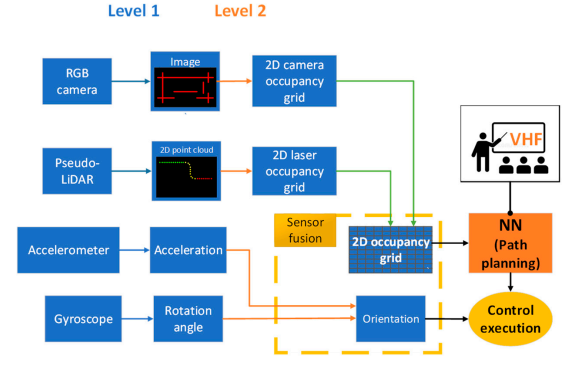
\includegraphics[width=0.65\textwidth]{gambar/arsitektur_sensor_fusion_umum.png}
\caption{Arsitektur umum sistem navigasi robot berbasis fusi sensor yang mengintegrasikan sensor visual, sensor jarak, dan sensor inersial untuk menghasilkan representasi lingkungan sebagai dasar perencanaan lintasan dan pengendalian robot (diadaptasi dari (\cite{Usinskis2025})).}
\label{fig:arsitektur_umum_sensor_fusion}
\end{figure}

Gambar~\ref{fig:arsitektur_umum_sensor_fusion} menunjukkan contoh arsitektur navigasi robot berbasis fusi sensor. Pada tingkat pertama (\textit{Level 1}), berbagai sensor seperti kamera, LiDAR, akselerometer, dan giroskop menghasilkan informasi sesuai karakteristik masing-masing. Informasi tersebut kemudian di\-proses menjadi representasi lingkungan yang lebih terstruktur pada tingkat kedua (\textit{Level 2}), seperti occupancy grid, estimasi orientasi, maupun fitur lingkungan lainnya. Selanjutnya, seluruh informasi digabungkan melalui mekanisme fusi sensor untuk membentuk model lingkungan yang digunakan oleh algoritma perencanaan lintasan dan pengendalian robot (\cite{Usinskis2025}).

Kualitas persepsi lingkungan memiliki pengaruh yang sangat besar terhadap performa navigasi robot. Informasi lingkungan yang tidak lengkap atau tidak akurat dapat menyebabkan kesalahan dalam proses pengambilan keputusan, menghasilkan lintasan yang tidak optimal, atau bahkan meningkatkan risiko terjadinya tabrakan. Oleh karena itu, pengembangan metode persepsi lingkungan dan fusi sensor menjadi salah satu topik penelitian yang paling aktif dalam bidang robotika bergerak otonom saat ini (\cite{Liu2024,Choi2023}).

Berdasarkan karakteristik tersebut, sistem navigasi robot modern tidak hanya berfokus pada perencanaan lintasan, tetapi juga pada kemampuan memperoleh representasi lingkungan yang akurat dan adaptif. Representasi lingkungan inilah yang selanjutnya menjadi dasar bagi berbagai metode navigasi dan penghindaran obstacle yang akan dibahas pada subbab-subbab berikutnya.

\subsection{Light Detection and Ranging (LiDAR)}

\textit{Light Detection and Ranging} (LiDAR) merupakan sensor aktif yang bekerja dengan memancarkan pulsa cahaya laser ke lingkungan sekitar dan mengukur waktu tempuh pantulan cahaya yang kembali menuju sensor. Informasi waktu tempuh tersebut digunakan untuk menghitung jarak antara sensor dan objek sehingga diperoleh representasi geometris lingkungan dalam bentuk kumpulan titik (\textit{point cloud}) maupun data jarak pada arah tertentu (\cite{Liu2024}).

LiDAR menjadi salah satu sensor yang paling banyak digunakan pada sistem navigasi robot otonom karena mampu menyediakan pengukuran jarak secara langsung dengan tingkat akurasi yang tinggi, laju pembaruan data yang cepat, serta relatif tidak terpengaruh oleh perubahan kondisi pencahayaan lingkungan (\cite{Macenski2022}). Karakteristik tersebut menjadikan LiDAR sangat sesuai untuk berbagai tugas persepsi robot, seperti pemetaan lingkungan, lokalisasi, deteksi obstacle, dan navigasi bergerak.

Prinsip dasar pengukuran jarak menggunakan LiDAR ditunjukkan pada Gambar~\ref{fig:lidar_principle}. Sensor memancarkan sinar laser menuju objek, kemudian mendeteksi pantulan cahaya yang kembali diterima oleh fotodetektor. Jarak objek dihitung berdasarkan waktu tempuh pulsa laser menggunakan prinsip \textit{time-of-flight} (ToF), yaitu:

\begin{equation}
d = \frac{c \times t}{2}
\label{eq:lidar_tof}
\end{equation}

dengan:

\begin{itemize}
\item $d$ adalah jarak objek terhadap sensor (m),
\item $c$ adalah kecepatan cahaya ($3 \times 10^{8}$ m/s),
\item $t$ adalah waktu tempuh pulsa laser pulang-pergi (s).
\end{itemize}

Melalui proses pengukuran tersebut, LiDAR dapat menentukan posisi objek berdasarkan jarak dan sudut pemindaian sehingga menghasilkan representasi spasial lingkungan yang digunakan oleh sistem navigasi robot.

\begin{figure}[H]
\centering
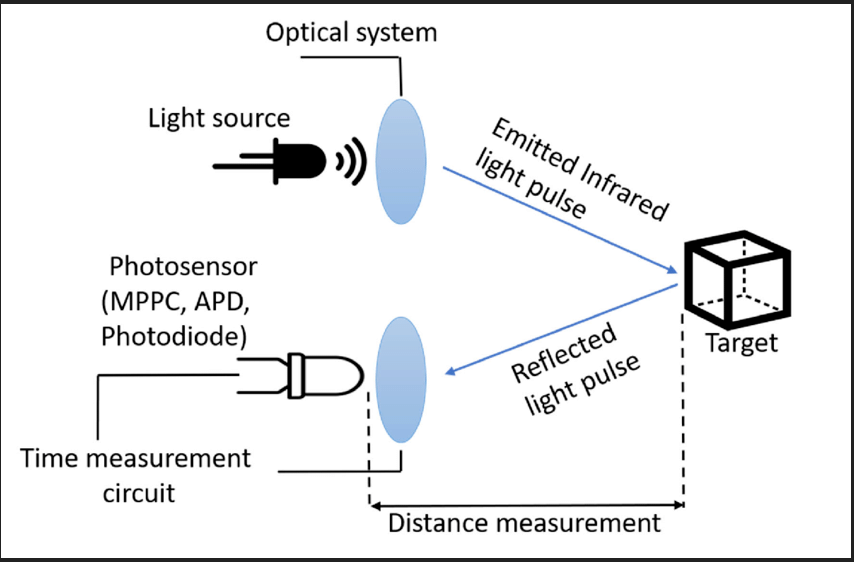
\includegraphics[width=0.4\textwidth]{gambar/fig_lidar_principle.png}
\caption{Prinsip pengukuran jarak menggunakan sensor LiDAR berbasis \textit{time-of-flight} serta representasi geometris lingkungan yang dihasilkan dari proses pemindaian (\cite{Pendse2024}).}
\label{fig:lidar_principle}
\end{figure}
Berdasarkan konfigurasi pemindaiannya, LiDAR dapat diklasifikasikan menjadi LiDAR dua dimensi (2D) dan LiDAR tiga dimensi (3D). LiDAR 3D melakukan pemindaian pada beberapa bidang vertikal secara simultan sehingga mampu menghasilkan representasi lingkungan yang lebih lengkap. Namun demikian, kebutuhan komputasi, konsumsi daya, dan biaya implementasinya relatif lebih tinggi dibandingkan LiDAR 2D (\cite{Fagundes2024}).

Sebaliknya, LiDAR 2D hanya melakukan pemindaian pada satu bidang horizontal sehingga menghasilkan informasi jarak dalam bentuk rangkaian titik hasil pengamatan pada bi\-dang tersebut. Meskipun memiliki keterbatasan dalam merepresentasikan struktur vertikal ling\-kungan, LiDAR 2D masih menjadi pilihan yang populer pada sistem robot bergerak karena sederhana, ekonomis, serta telah didukung secara luas oleh berbagai paket navigasi berbasis ROS (\cite{Macenski2022}).

Contoh hasil pemindaian LiDAR ditunjukkan pada Gambar~\ref{fig:lidar_2d_scan}. Data hasil pengamatan direpresentasikan sebagai kumpulan titik yang menggambarkan struktur lingkungan di sekitar sensor. Distribusi titik yang dihasilkan dapat bervariasi bergantung pada karakteristik objek, jarak pengamatan, sudut pantulan, dan kondisi lingkungan sehingga menghasilkan kepadatan data yang tidak selalu seragam.

\begin{figure}[H]
\centering
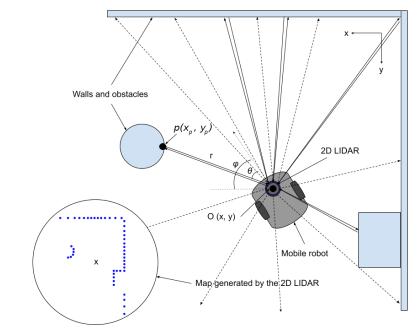
\includegraphics[width=0.4\textwidth]{gambar/fig_lidar_2d_scan.png}
\caption{Contoh representasi lingkungan yang diperoleh dari hasil pemindaian LiDAR dalam bentuk point cloud (\cite{Bouazizi2023}).}
\label{fig:lidar_2d_scan}
\end{figure}

Meskipun memiliki akurasi pengukuran yang tinggi, LiDAR 2D memiliki keterbatasan karena hanya mengamati lingkungan pada satu bidang horizontal. Akibatnya, sebagian objek dapat berada di luar bidang pemindaian sehingga tidak menghasilkan informasi yang memadai bagi sistem navigasi. Keterbatasan ini sering dikaitkan dengan fenomena \textit{blind spot} dan daerah dengan kepadatan titik yang rendah (\textit{low-density region}) (\cite{Kibii2022,Fagundes2024}).

Gambar~\ref{fig:fig_lidar_blindspot} menunjukkan contoh area \textit{blind spot} dan daerah dengan kepadatan titik rendah pada hasil pengamatan LiDAR. Pada area tersebut, jumlah pantulan laser yang diterima sensor menjadi terbatas sehingga representasi objek tidak terbentuk secara lengkap. Kondisi ini dapat menyebabkan obstacle tertentu sulit dikenali atau bahkan tidak terdeteksi, terutama ketika objek memiliki dimensi kecil, posisi yang kurang menguntungkan terhadap sensor, atau berada di luar bidang pemindaian utama.

\begin{figure}[H]
\centering
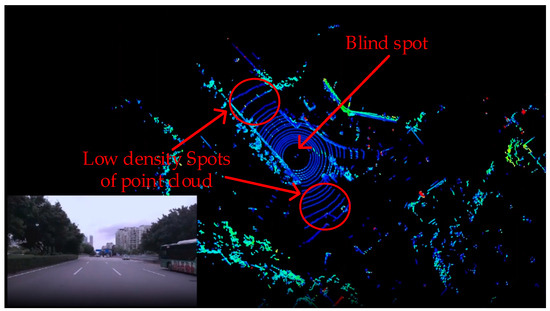
\includegraphics[width=0.5\textwidth]{gambar/fig_lidar_blindspot.png}
\caption{Contoh area \textit{blind spot} dan daerah dengan kepadatan point cloud rendah pada hasil pengamatan LiDAR (\cite{Xie2024}).}
\label{fig:fig_lidar_blindspot}
\end{figure}

Berbagai penelitian telah mengusulkan penggunaan sensor tambahan untuk mengatasi keterbatasan tersebut, salah satunya melalui integrasi LiDAR dengan kamera visual maupun kamera termal (\cite{Choi2023,Schichler2025}). Pendekatan multisensor memungkinkan sistem memperoleh informasi lingkungan yang tidak dapat diamati secara optimal oleh LiDAR sehingga meningkatkan kualitas persepsi, deteksi obstacle, dan keselamatan navigasi robot.

Pada penelitian ini, LiDAR 2D digunakan sebagai sensor utama untuk memperoleh informasi jarak obstacle di sekitar robot. Namun demikian, keterbatasan pemindaian pada area \textit{blind spot} serta kemungkinan hilangnya informasi objek tertentu menjadi alasan penggunaan kamera termal sebagai sensor pelengkap. Informasi dari kedua sensor kemudian dikombinasikan untuk menghasilkan representasi lingkungan yang lebih lengkap dan mendukung proses navigasi robot secara lebih robust.

\subsection{Kamera Termal}

Kamera termal merupakan sensor pasif yang bekerja dengan mendeteksi radiasi inframerah yang dipancarkan oleh objek dan mengubahnya menjadi representasi citra berdasarkan distribusi temperatur permukaan. Berbeda dengan kamera RGB yang bergantung pada cahaya tampak, kamera termal mampu menghasilkan informasi visual berdasarkan energi panas sehingga tetap dapat beroperasi pada kondisi pencahayaan rendah maupun lingkungan yang minim cahaya (\cite{Choi2023,Schichler2025}).

Pada spektrum elektromagnetik, radiasi inframerah terletak di luar rentang cahaya tampak yang dapat diamati oleh mata manusia. Seluruh objek dengan temperatur di atas nol absolut memancarkan energi termal dalam jumlah tertentu. Intensitas radiasi tersebut dipengaruhi oleh temperatur permukaan objek sehingga dapat dimanfaatkan untuk membedakan objek yang memiliki karakteristik termal berbeda (\cite{Castro2016}).

\begin{figure}[H]
\centering
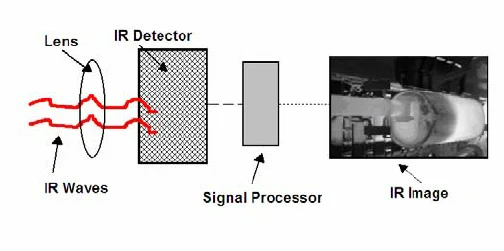
\includegraphics[width=0.75\textwidth]{gambar/fig_thermal_principle.png}
\caption{Prinsip pembentukan citra termal melalui deteksi radiasi inframerah yang dipancarkan objek dan diproses menjadi representasi visual temperatur (diadaptasi dari (\cite{Koschan2006})).}
\label{fig:thermal_principle}
\end{figure}

Gambar~\ref{fig:thermal_principle} menunjukkan prinsip dasar pembentukan citra termal. Energi inframerah yang dipancarkan oleh objek ditangkap oleh sensor termal dan dikonversi menjadi nilai intensitas piksel. Nilai tersebut kemudian divisualisasikan dalam bentuk citra grayscale maupun \textit{false color} untuk mempermudah interpretasi kondisi termal lingkungan.

Dalam sistem robotika dan kendaraan otonom, kamera termal banyak dimanfaatkan untuk meningkatkan kemampuan persepsi lingkungan, terutama pada kondisi yang menantang bagi kamera konvensional. Berbagai penelitian menunjukkan bahwa informasi termal dapat digunakan untuk deteksi manusia, deteksi obstacle, segmentasi lingkungan, serta meningkatkan robustitas sistem persepsi ketika kondisi pencahayaan berubah secara signifikan (\cite{Castro2016,Choi2023,Schichler2025}).

Dibandingkan kamera RGB, kamera termal memiliki keunggulan karena tidak bergantung pada intensitas cahaya tampak. Objek yang memiliki perbedaan temperatur terhadap lingkungan sekitar umumnya tetap dapat diamati meskipun berada pada kondisi malam hari atau area dengan pencahayaan terbatas. Karakteristik tersebut menjadikan kamera termal sebagai sensor pelengkap yang menarik untuk dikombinasikan dengan LiDAR pada sistem navigasi robot otonom.

Meskipun demikian, kamera termal juga memiliki beberapa keterbatasan. Informasi yang diperoleh umumnya hanya merepresentasikan distribusi temperatur permukaan tanpa memberikan informasi jarak secara langsung. Selain itu, kualitas citra termal dapat dipengaruhi oleh kondisi lingkungan, emissivitas material, serta perbedaan temperatur antara objek dan latar belakang (\cite{Schichler2025}). Oleh karena itu, data termal umumnya memerlukan tahap pemrosesan lanjutan agar dapat dimanfaatkan secara efektif dalam sistem navigasi robot.

Salah satu pendekatan yang banyak digunakan untuk mengekstraksi informasi lingkungan dari citra termal adalah segmentasi semantik (\textit{semantic segmentation}). Segmentasi semantik merupakan proses klasifikasi setiap piksel citra ke dalam kelas tertentu sehingga diperoleh representasi lingkungan yang lebih terstruktur (\cite{Sirmacek2019}). Melalui proses ini, sistem dapat membedakan area yang dapat dilalui (\textit{traversable area}) dan area yang tidak dapat dilalui (\textit{non-traversable area}) berdasarkan karakteristik visual yang diamati.

Secara umum, fungsi segmentasi semantik dapat dinyatakan sebagai:

\begin{equation}
f : I \rightarrow C
\label{eq:semantic_segmentation}
\end{equation}

dengan:

\begin{itemize}
\item $I$ adalah citra masukan;
\item $C$ adalah himpunan kelas yang tersedia;
\item $f$ adalah fungsi klasifikasi piksel.
\end{itemize}

Keluaran proses segmentasi berupa peta kelas (\textit{semantic mask}) yang memiliki dimensi sama dengan citra masukan. Setiap piksel pada peta tersebut merepresentasikan kategori objek tertentu sesuai hasil prediksi model. Informasi tersebut selanjutnya dapat digunakan untuk mengidentifikasi obstacle, area bebas, maupun batas lintasan yang relevan terhadap proses navigasi robot.

\begin{figure}[H]
\centering
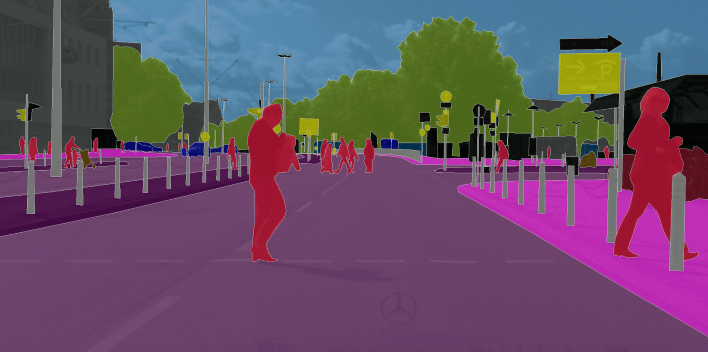
\includegraphics[width=0.8\textwidth]{gambar/fig_semantic_segmentation.png}
\caption{Contoh hasil segmentasi semantik yang mengklasifikasikan setiap piksel citra ke dalam kelas objek tertentu (diadaptasi dari (\cite{Sirmacek2019})).}
\label{fig:semantic_segmentation}
\end{figure}

Gambar~\ref{fig:semantic_segmentation} menunjukkan contoh keluaran segmentasi semantik berupa \textit{semantic mask} yang mengelompokkan setiap piksel ke dalam kelas objek tertentu. Representasi tersebut memberikan informasi lingkungan yang lebih mudah diinterpretasikan dibandingkan citra mentah sehingga dapat dimanfaatkan sebagai dasar pengambilan keputusan navigasi.

Pada penelitian ini, citra termal diproses melalui tahapan segmentasi semantik untuk membedakan area yang dapat dilalui (\textit{traversable area}) dan area yang mengandung obstacle (\textit{non-traversable area}) berdasarkan karakteristik termal yang diamati sensor. Informasi hasil segmentasi tersebut digunakan untuk membentuk traversability termal yang selanjutnya dikombinasikan dengan informasi LiDAR melalui proses fusi sensor. Integrasi kedua sumber informasi tersebut diharapkan mampu menghasilkan representasi lingkungan yang lebih lengkap dan meningkatkan kemampuan robot dalam mendeteksi obstacle yang berada pada area \textit{blind-spot} LiDAR.
\subsection{Fusi Sensor}

Fusi sensor (\textit{sensor fusion}) merupakan proses penggabungan informasi yang diperoleh dari beberapa sensor untuk menghasilkan representasi lingkungan yang lebih akurat, lengkap, dan andal dibandingkan penggunaan sensor tunggal (\cite{Khaleghi2013}). Pada sistem robot bergerak otonom, fusi sensor banyak digunakan untuk meningkatkan kualitas persepsi lingkungan, mengurangi ketidakpastian pengukuran, serta meningkatkan robustitas sistem terhadap keterbatasan masing-masing sensor.

Penggunaan sensor tunggal sering kali tidak mampu menyediakan informasi lingkungan secara menyeluruh. Sebagai contoh, LiDAR mampu menghasilkan informasi geometris dan jarak dengan akurasi tinggi, namun memiliki keterbatasan dalam mengenali karakteristik visual objek serta rentan terhadap area \textit{blind-spot}. Sebaliknya, kamera mampu menyediakan informasi visual yang kaya, tetapi tidak dapat mengukur jarak secara langsung dengan tingkat akurasi yang setara dengan LiDAR. Oleh karena itu, kombinasi beberapa sensor sering digunakan untuk memperoleh keunggulan dari masing-masing sensor sekaligus mengurangi kelemahannya (\cite{Khaleghi2013,Choi2023}).

Secara umum, proses fusi sensor dapat dinyatakan sebagai:

\begin{equation}
Z_f = F(Z_1,Z_2,\dots,Z_n)
\label{eq:sensor_fusion}
\end{equation}

dengan:

\begin{itemize}
\item $Z_f$ adalah informasi hasil fusi;
\item $Z_i$ adalah informasi yang diperoleh dari sensor ke-$i$;
\item $F(\cdot)$ adalah fungsi fusi yang digunakan.
\end{itemize}

Berdasarkan tingkat pengolahan data, fusi sensor umumnya dibedakan menjadi tiga kategori utama, yaitu \textit{data-level fusion}, \textit{feature-level fusion}, dan \textit{decision-level fusion} (\cite{Khaleghi2013,Debie2019}).

\begin{enumerate}
\item \textbf{Data-Level Fusion}

Pada pendekatan ini, penggabungan dilakukan langsung terhadap data mentah yang diperoleh dari sensor sebelum dilakukan proses ekstraksi fitur. Karena memanfaatkan informasi sensor secara penuh, pendekatan ini berpotensi menghasilkan representasi lingkungan yang sangat kaya. Namun demikian, metode ini membutuhkan sinkronisasi spasial dan temporal yang ketat serta sumber daya komputasi yang relatif tinggi.

\item \textbf{Feature-Level Fusion}

Pada \textit{feature-level fusion}, masing-masing sensor terlebih dahulu diproses untuk menghasilkan fitur-fitur tertentu. Fitur tersebut kemudian digabungkan untuk membentuk representasi lingkungan yang lebih informatif. Pendekatan ini mampu mengurangi volume data yang diproses dibandingkan \textit{data-level fusion}, tetapi tetap memerlukan kesesuaian representasi fitur antar sensor.

\item \textbf{Decision-Level Fusion}

Pada pendekatan ini, setiap sensor menghasilkan keputusan atau interpretasi lingkungan secara independen. Hasil keputusan tersebut kemudian digabungkan untuk memperoleh keputusan akhir sistem. Dibandingkan dua pendekatan sebelumnya, \textit{decision-level fusion} memiliki kompleksitas implementasi yang lebih rendah dan lebih fleksibel untuk mengintegrasikan sensor yang memiliki karakteristik berbeda.
\end{enumerate}

\begin{figure}[H]
\centering
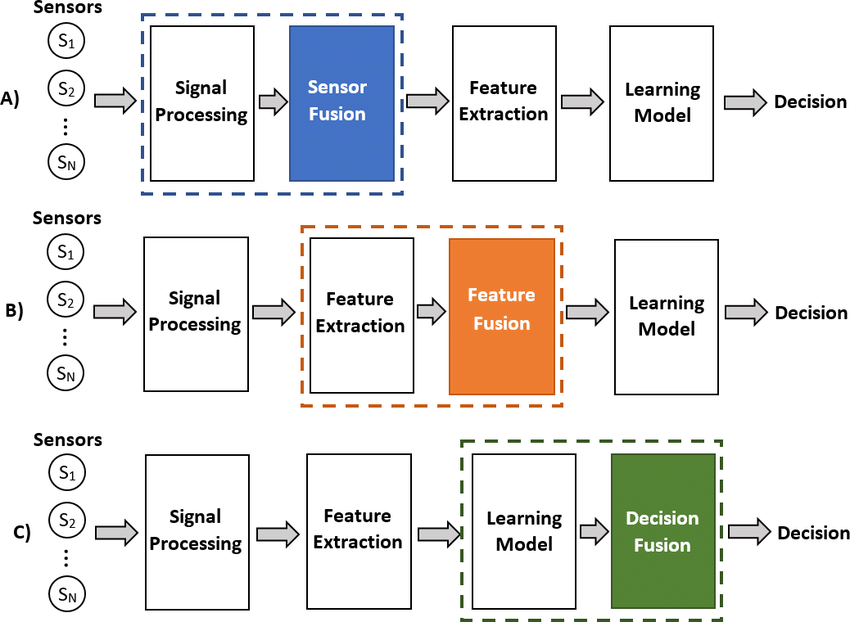
\includegraphics[width=0.75\textwidth]{gambar/fig_sensor_fusion_levels.png}
\caption{Tiga tingkatan umum fusi informasi, yaitu \textit{data-level fusion}, \textit{feature-level fusion}, dan \textit{decision-level fusion} (diadaptasi dari (\cite{Debie2019})).}
\label{fig:sensor_fusion_levels}
\end{figure}

Gambar~\ref{fig:sensor_fusion_levels} memperlihatkan tiga tingkatan utama fusi informasi yang umum digunakan pada sistem multisensor. Pada \textit{data-level fusion}, proses penggabungan dilakukan sebelum ekstraksi fitur. Pada \textit{feature-level fusion}, data dari masing-masing sensor terlebih dahulu diubah menjadi fitur tertentu sebelum digabungkan. Sementara itu, \textit{decision-level fusion} melakukan penggabungan setelah masing-masing sensor menghasilkan interpretasi atau keputusan terhadap lingkungan yang diamati (\cite{Debie2019,Khaleghi2013}).

Dalam bidang robotika, kombinasi LiDAR dan kamera merupakan salah satu pendekatan fusi sensor yang paling banyak digunakan karena kedua sensor tersebut memiliki karakteristik yang saling melengkapi. LiDAR menyediakan informasi geometris lingkungan secara akurat, sedangkan kamera menyediakan informasi visual yang kaya mengenai objek dan kondisi lingkungan (\cite{Choi2023,Schichler2025}). Integrasi kedua sensor tersebut telah banyak dimanfaatkan untuk navigasi robot otonom, deteksi obstacle, pemetaan lingkungan, serta sistem bantuan pengemudi pada kendaraan cerdas.

Pada penelitian ini, fusi sensor dilakukan antara informasi traversability yang diperoleh dari LiDAR dan informasi traversability yang diperoleh dari citra termal hasil segmentasi semantik. Masing-masing sensor terlebih dahulu diproses secara independen untuk menghasilkan nilai traversability yang merepresentasikan tingkat kelayakan suatu area untuk dilalui robot. Selanjutnya, kedua informasi tersebut digabungkan untuk menghasilkan traversability efektif yang digunakan sebagai masukan sistem navigasi.

Berdasarkan klasifikasi yang telah dijelaskan sebelumnya, pendekatan yang digunakan dalam penelitian ini termasuk ke dalam \textit{decision-level fusion}. Hal ini disebabkan karena proses penggabungan dilakukan setelah masing-masing sensor menghasilkan interpretasi lingkungan dalam bentuk informasi traversability, bukan pada data mentah maupun fitur hasil ekstraksi. Pendekatan tersebut dipilih karena lebih sederhana untuk diimplementasikan pada lingkungan robot bergerak berbasis ROS serta tidak memerlukan proses kalibrasi spasial yang kompleks sebagaimana pada \textit{data-level fusion} dan \textit{feature-level fusion}.

Melalui pendekatan ini, sistem dapat memanfaatkan keunggulan LiDAR dalam pengukuran jarak sekaligus memanfaatkan kemampuan kamera termal dalam mendeteksi obstacle yang berada di luar bidang pemindaian LiDAR. Dengan demikian, representasi lingkungan yang dihasilkan menjadi lebih lengkap sehingga diharapkan mampu meningkatkan keselamatan navigasi, khususnya ketika robot menghadapi obstacle berprofil rendah yang berada pada area \textit{blind-spot} LiDAR.

\subsection{Analisis Traversability}

Traversability merupakan ukuran yang menggambarkan tingkat kelayakan suatu area untuk dilalui oleh robot berdasarkan kondisi lingkungan yang diamati. Konsep traversability banyak digunakan pada sistem navigasi robot bergerak dan kendaraan otonom untuk membantu proses pengambilan keputusan terkait pemilihan lintasan yang aman dan efisien (\cite{Scherer2008,Howard2017}). Melalui analisis traversability, sistem tidak hanya mengetahui keberadaan obstacle, tetapi juga dapat mengevaluasi tingkat risiko yang dimiliki setiap area di sekitar robot.

Secara umum, nilai traversability dapat dipengaruhi oleh berbagai faktor lingkungan, se\-perti keberadaan obstacle, jarak terhadap obstacle, lebar ruang bebas yang tersedia, kemiringan permukaan, kondisi medan, maupun tingkat ketidakpastian hasil pengukuran sensor (\cite{Scherer2008}). Area yang memiliki risiko rendah umumnya diberikan nilai traversability tinggi, sedangkan area yang berpotensi menyebabkan tabrakan atau menghambat pergerakan robot diberikan nilai traversability yang lebih rendah.

Secara matematis, traversability dapat direpresentasikan sebagai suatu fungsi:

\begin{equation}
T = f(x)
\label{eq:traversability_general}
\end{equation}

dengan:

\begin{itemize}
\item $T$ adalah nilai traversability;
\item $x$ adalah parameter lingkungan yang digunakan dalam proses evaluasi.
\end{itemize}

Nilai traversability biasanya dinormalisasi ke dalam rentang tertentu, misalnya antara 0 dan 1. Nilai mendekati 1 menunjukkan area yang aman untuk dilalui, sedangkan nilai mendekati 0 menunjukkan area yang tidak direkomendasikan untuk dilalui robot.

Pada sistem navigasi modern, traversability sering digunakan sebagai representasi tingkat keamanan lingkungan karena mampu mengubah informasi sensor yang kompleks menjadi parameter yang lebih mudah digunakan oleh algoritma navigasi (\cite{Howard2017}). Dengan pendekatan ini, robot dapat memilih perilaku navigasi yang berbeda ketika menghadapi kondisi lingkungan yang aman maupun berisiko.

\begin{figure}[H]
\centering
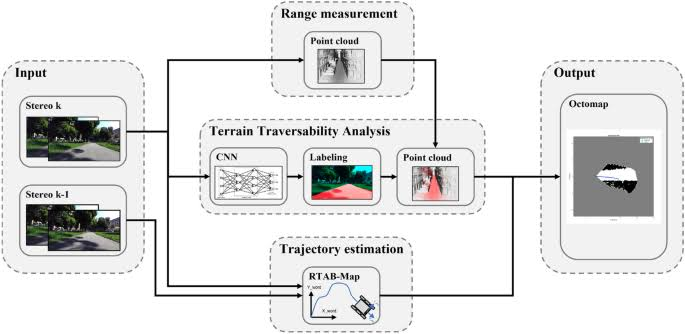
\includegraphics[width=0.8\textwidth]{gambar/fig_traversability_concept.jpeg}
\caption{Ilustrasi proses pembentukan informasi traversability dari data sensor melalui analisis lingkungan dan representasi spasial untuk mendukung navigasi robot otonom (diadaptasi dari (\cite{Polato2025})).}
\label{fig:traversability_concept}
\end{figure}

Pada penelitian ini, traversability digunakan sebagai representasi utama kondisi lingkungan yang diamati oleh robot. Nilai traversability diperoleh dari dua sumber informasi yang berbeda, yaitu LiDAR dan kamera termal. Masing-masing sensor menghasilkan estimasi trav\-ersability secara independen berdasarkan karakteristik pengamatan yang dimiliki.

LiDAR menghasilkan traversability berdasarkan informasi geometris lingkungan yang di\-peroleh dari hasil pemindaian jarak obstacle di sekitar robot. Informasi tersebut memungkinkan sistem untuk mengevaluasi ketersediaan ruang bebas dan tingkat kedekatan robot terhadap obstacle. Secara umum, semakin besar ruang bebas yang tersedia dan semakin jauh obstacle berada dari robot, maka nilai traversability yang dihasilkan akan semakin tinggi.

Sementara itu, kamera termal menghasilkan traversability melalui proses segmentasi semantik terhadap citra termal. Hasil segmentasi digunakan untuk mengidentifikasi area yang dapat dilalui (\textit{traversable area}) dan area yang mengandung obstacle (\textit{non-traversable area}). Pendekatan ini memungkinkan sistem memperoleh informasi lingkungan yang tidak sepenuhnya dapat diamati oleh LiDAR, khususnya pada kasus obstacle berprofil rendah yang berada di luar bidang pemindaian sensor.

Karena masing-masing sensor memiliki karakteristik yang berbeda, kedua nilai traversability tersebut kemudian dikombinasikan melalui proses fusi sensor untuk menghasilkan traver\-sability efektif. Traversability efektif inilah yang digunakan sebagai representasi akhir kondisi lingkungan dan menjadi masukan utama bagi sistem navigasi berbasis \textit{Artificial Potential Field} (APF) dan logika fuzzy Mamdani.

Dengan menggunakan traversability sebagai parameter utama, sistem tidak hanya mempertimbangkan keberadaan obstacle, tetapi juga mempertimbangkan tingkat keamanan lingkungan secara keseluruhan. Pendekatan tersebut memungkinkan robot menyesuaikan perilaku navigasi secara lebih adaptif ketika menghadapi kondisi lingkungan yang memiliki tingkat risiko berbeda.

\subsection{Artificial Potential Field}

\textit{Artificial Potential Field} (APF) merupakan salah satu metode perencanaan lintasan reaktif yang banyak digunakan pada sistem navigasi robot bergerak karena memiliki struktur yang sederhana, kebutuhan komputasi yang relatif rendah, serta mampu menghasilkan respons navigasi secara \textit{real-time} (\cite{Khatib1986,Ge2002}). Pada metode ini, lingkungan direpresentasikan sebagai medan potensial virtual yang terdiri atas gaya tarik menuju tujuan (\textit{attractive potential}) dan gaya tolak dari obstacle (\textit{repulsive potential}).

Konsep APF pertama kali diperkenalkan oleh Khatib (\cite{Khatib1986}) dengan memodelkan robot sebagai partikel yang bergerak di dalam medan potensial. Tujuan navigasi menghasilkan gaya atraktif yang menarik robot menuju target, sedangkan obstacle menghasilkan gaya repulsif yang mendorong robot menjauhi area berbahaya. Interaksi kedua gaya tersebut menentukan arah pergerakan robot pada setiap waktu.

Secara matematis, fungsi potensial total dapat dinyatakan sebagai:

\begin{equation}
U(q)=U_{att}(q)+U_{rep}(q)
\label{eq:apf_total}
\end{equation}

dengan $U(q)$ merupakan potensial total, $U_{att}(q)$ merupakan potensial atraktif, $U_{rep}(q)$ mer\-upakan potensial repulsif, dan $q$ merupakan posisi robot.

Potensial atraktif yang menarik robot menuju tujuan dapat dirumuskan sebagai:

\begin{equation}
U_{att}(q)=\frac{1}{2}k_{att}\|q-q_g\|^2
\label{eq:apf_attractive}
\end{equation}

dengan $k_{att}$ merupakan koefisien gaya tarik dan $q_g$ merupakan posisi tujuan. Berdasarkan fungsi tersebut, gaya atraktif diperoleh melalui gradien negatif potensial sebagai:

\begin{equation}
F_{att}(q)=-\nabla U_{att}(q)
\label{eq:f_att}
\end{equation}

Sementara itu, obstacle menghasilkan potensial repulsif yang dapat dituliskan sebagai:

\begin{equation}
U_{rep}(q)=
\begin{cases}
\frac{1}{2}k_{rep}
\left(
\frac{1}{\rho(q)}
-\frac{1}{\rho_0}
\right)^2,
&
\rho(q)\leq\rho_0
\\
0,
&
\rho(q)>\rho_0
\end{cases}
\label{eq:apf_repulsive}
\end{equation}

dengan $k_{rep}$ merupakan koefisien gaya tolak, $\rho(q)$ merupakan jarak robot terhadap obstacle, dan $\rho_0$ merupakan radius pengaruh obstacle. Gaya repulsif kemudian diperoleh melalui:

\begin{equation}
F_{rep}(q)=-\nabla U_{rep}(q)
\label{eq:f_rep}
\end{equation}

Kombinasi gaya atraktif dan repulsif menghasilkan gaya total yang menentukan arah pergerakan robot, yaitu:

\begin{equation}
F(q)=F_{att}(q)+F_{rep}(q)
\label{eq:f_total}
\end{equation}

Arah vektor $F(q)$ selanjutnya digunakan sebagai dasar pembentukan perintah navigasi robot.

Metode APF memiliki beberapa keunggulan, antara lain implementasi yang sederhana, kebutuhan komputasi yang rendah, serta kemampuan menghasilkan perilaku penghindaran obstacle secara cepat. Karakteristik tersebut menjadikan APF banyak digunakan pada sistem navigasi robot bergerak yang membutuhkan respons reaktif terhadap perubahan kondisi lingkungan (\cite{Ge2002,Zhang2023}).

Meskipun demikian, APF juga memiliki beberapa keterbatasan. Salah satu permasalahan yang paling dikenal adalah \textit{local minima}, yaitu kondisi ketika gaya atraktif dan gaya repulsif saling meniadakan sehingga robot berhenti sebelum mencapai tujuan. Selain itu, penggunaan parameter atraktif dan repulsif yang bernilai tetap menyebabkan perilaku navigasi kurang adaptif terhadap perubahan tingkat risiko lingkungan (\cite{Ge2002,Zhang2023}).

Untuk mengatasi keterbatasan tersebut, berbagai penelitian mengintegrasikan APF dengan metode kecerdasan komputasional, salah satunya logika fuzzy, sehingga parameter navigasi dapat disesuaikan secara dinamis berdasarkan kondisi lingkungan yang diamati robot (\cite{Masehian2010,Zhang2023}).

Pada penelitian ini, APF digunakan sebagai mekanisme navigasi lokal yang menghasilkan perilaku penghindaran obstacle secara reaktif. Nilai parameter navigasi tidak ditetapkan secara tetap, melainkan disesuaikan secara adaptif menggunakan logika fuzzy berdasarkan informasi traversability hasil fusi LiDAR dan kamera termal. Pendekatan tersebut diharapkan mampu meningkatkan keselamatan navigasi ketika robot beroperasi pada lingkungan yang mengandung obstacle berprofil rendah maupun obstacle dinamis.

\subsection{Logika Fuzzy Mamdani}

Logika fuzzy merupakan metode kecerdasan komputasional yang diperkenalkan oleh Za\-deh pada tahun 1965 untuk merepresentasikan ketidakpastian dan penalaran yang menyerupai cara berpikir manusia (\cite{Zadeh1965}). Berbeda dengan logika biner yang hanya mengenal nilai benar atau salah, logika fuzzy memungkinkan suatu variabel memiliki derajat keanggotaan pada rentang kontinu antara 0 dan 1. Karakteristik tersebut menjadikan logika fuzzy banyak digunakan pada sistem kendali dan pengambilan keputusan yang melibatkan informasi tidak pasti atau sulit dimodelkan secara matematis (\cite{Mendel1995,Ross2010}).

Pada sistem navigasi robot bergerak, logika fuzzy sering digunakan untuk menghubungkan informasi sensor dengan keputusan navigasi tanpa memerlukan model lingkungan yang kompleks. Pendekatan ini memungkinkan robot menghasilkan respons yang lebih adaptif terhadap perubahan kondisi lingkungan dibandingkan metode berbasis parameter tetap (\cite{Masehian2010,Haider2022}).

Secara umum, sistem inferensi fuzzy terdiri atas empat tahapan utama, yaitu \textit{fuzzification}, basis aturan (\textit{rule base}), mesin inferensi (\textit{inference engine}), dan \textit{defuzzification}, sebagaimana ditunjukkan pada Gambar~\ref{fig:fuzzy_system}.

\begin{figure}[H]
\centering
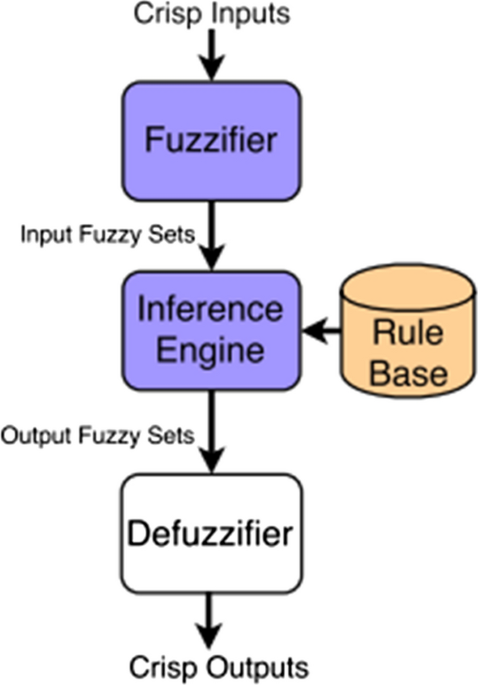
\includegraphics[width=0.45\textwidth]{gambar/fig_fuzzy_system.png}
\caption{Struktur umum sistem inferensi fuzzy Mamdani yang terdiri atas proses fuzzifikasi, basis aturan (\textit{rule base}), mesin inferensi (\textit{inference engine}), dan defuzzifikasi untuk menghasilkan keluaran tegas (\textit{crisp output}) dari masukan tegas (\textit{crisp input}) (diadaptasi dari (\cite{Ross2010,Kambalimath2020})).}
\label{fig:fuzzy_system}
\end{figure}

Tahap pertama adalah fuzzifikasi, yaitu proses transformasi nilai masukan tegas (\textit{crisp input}) menjadi derajat keanggotaan pada himpunan fuzzy tertentu. Derajat keanggotaan direpresentasikan menggunakan fungsi keanggotaan (\textit{membership function}) yang nilainya berada pada rentang:

\begin{equation}
0 \leq \mu(x) \leq 1
\label{eq:fuzzy_membership}
\end{equation}

dengan $\mu(x)$ menyatakan derajat keanggotaan suatu nilai $x$ terhadap himpunan fuzzy tertentu. Salah satu fungsi keanggotaan yang paling banyak digunakan adalah fungsi segitiga (\textit{triangular membership function}) yang dirumuskan sebagai:

\begin{equation}
\mu(x)=
\begin{cases}
0, & x \leq a \\
\dfrac{x-a}{b-a}, & a < x \leq b \\
\dfrac{c-x}{c-b}, & b < x < c \\
0, & x \geq c
\end{cases}
\label{eq:triangular_mf}
\end{equation}

dengan $a$, $b$, dan $c$ merupakan parameter fungsi keanggotaan.

Setelah proses fuzzifikasi, sistem melakukan inferensi berdasarkan sekumpulan aturan linguistik berbentuk \textit{IF--THEN}. Metode Mamdani merupakan salah satu metode inferensi fuzzy yang paling banyak digunakan karena memiliki struktur yang intuitif dan mudah dipahami (\cite{Mamdani1975}). Secara umum, aturan fuzzy dapat dituliskan sebagai:

\begin{equation}
\text{IF } A \text{ AND } B \text{ THEN } C
\label{eq:fuzzy_rule}
\end{equation}

dengan $A$ dan $B$ merupakan kondisi masukan, sedangkan $C$ merupakan keluaran yang dihasilkan. Pada proses inferensi, operator logika fuzzy digunakan untuk menentukan tingkat aktivasi setiap aturan. Untuk operator AND, nilai aktivasi umumnya dihitung menggunakan operator minimum:

\begin{equation}
\alpha = \min(\mu_A,\mu_B)
\label{eq:min_operator}
\end{equation}

dengan $\alpha$ merupakan kekuatan aktivasi aturan (\textit{firing strength}).

Tahap terakhir adalah defuzzifikasi, yaitu proses mengubah keluaran fuzzy menjadi nilai tegas yang dapat digunakan oleh sistem kendali. Metode yang paling umum digunakan adalah metode centroid karena menghasilkan keluaran yang halus dan stabil (\cite{Ross2010}). Nilai keluaran hasil defuzzifikasi centroid dapat dihitung menggunakan:

\begin{equation}
z^*=
\frac{
\int z , \mu(z), dz
}{
\int \mu(z), dz
}
\label{eq:centroid}
\end{equation}

dengan $z^*$ merupakan keluaran tegas hasil defuzzifikasi dan $\mu(z)$ merupakan fungsi keanggotaan keluaran.

Metode Mamdani banyak digunakan pada sistem navigasi robot karena mampu menerjemahkan pengetahuan heuristik manusia ke dalam bentuk aturan yang mudah diimplementasikan. Selain itu, metode ini memiliki kemampuan adaptasi yang baik ketika informasi sensor bersifat tidak pasti atau berubah secara dinamis (\cite{Benaicha2026,Masehian2010}).

Pada penelitian ini, logika fuzzy Mamdani digunakan untuk menyesuaikan parameter navigasi berdasarkan kondisi lingkungan yang diamati robot. Variabel masukan yang digunakan adalah jarak obstacle terdekat dan nilai \textit{effective traversability} hasil fusi LiDAR dan kamera termal. Sementara itu, variabel keluaran berupa \textit{repulsive gain} dan \textit{speed scale} yang digunakan untuk mengatur perilaku navigasi APF secara adaptif. Dengan pendekatan tersebut, robot diharapkan mampu mempertahankan margin keselamatan yang lebih baik ketika beroperasi pada lingkungan yang mengandung obstacle berprofil rendah maupun obstacle dinamis.

\subsection{Robot Operating System (ROS), Navigation Stack, dan Gazebo}

Robot Operating System (ROS) merupakan \textit{middleware} sumber terbuka yang banyak digunakan dalam pengembangan sistem robotika modern. ROS menyediakan mekanisme komunikasi antarproses, pustaka perangkat lunak, serta berbagai alat pengembangan yang memungkinkan integrasi sensor, aktuator, dan algoritma robotika dalam satu sistem yang modular (\cite{Quigley2009,Macenski2022}).

Pada ROS, setiap fungsi sistem dijalankan dalam bentuk \textit{node} yang saling berkomunikasi melalui mekanisme \textit{topic}, \textit{service}, dan \textit{action}. Pendekatan ini memungkinkan proses akuisisi data sensor, pemrosesan informasi, perencanaan lintasan, serta pengendalian robot dilakukan secara terdistribusi dan terintegrasi dalam satu kerangka kerja yang konsisten (\cite{Quigley2009}).

Salah satu paket yang banyak digunakan pada aplikasi navigasi robot bergerak adalah \textit{ROS Navigation Stack}. Paket ini menyediakan berbagai komponen yang mendukung proses lokalisasi, pengelolaan peta lingkungan, perencanaan lintasan, penghindaran obstacle, dan pengendalian gerak robot (\cite{Macenski2022}). Melalui integrasi komponen-komponen tersebut, robot dapat bergerak secara otonom menuju tujuan yang diberikan sambil mempertimbangkan kondisi lingkungan di sekitarnya.

Pada penelitian ini, perencanaan lintasan global dilakukan menggunakan \textit{NavfnROS}. Paket ini mengimplementasikan algoritma Dijkstra untuk mencari lintasan dengan biaya minimum berdasarkan informasi yang tersimpan pada \textit{costmap} (\cite{Brock2009}). Algoritma tersebut bekerja dengan menghitung biaya kumulatif dari setiap simpul yang dapat dilalui hingga diperoleh lintasan optimum menuju tujuan.

Secara umum, proses pencarian lintasan minimum pada algoritma Dijkstra dapat dinyatakan sebagai:

\begin{equation}
d(v)=\min_{u \in V}
\left[
d(u)+w(u,v)
\right]
\label{eq:dijkstra}
\end{equation}

dengan $d(v)$ menyatakan biaya minimum menuju simpul $v$, $d(u)$ merupakan biaya minimum menuju simpul sebelumnya, $w(u,v)$ merupakan biaya perpindahan antar simpul, dan $V$ adalah himpunan simpul pada peta navigasi.

Meskipun mampu menghasilkan lintasan global yang optimal, NavfnROS tidak secara langsung menangani perubahan kondisi lingkungan yang terjadi secara lokal selama robot bergerak. Oleh karena itu, diperlukan mekanisme navigasi lokal yang mampu merespons obstacle secara real-time. Pada penelitian ini, fungsi tersebut direalisasikan menggunakan metode Artificial Potential Field (APF) yang dikombinasikan dengan logika fuzzy Mamdani.

Selain ROS, penelitian ini juga memanfaatkan Gazebo sebagai lingkungan simulasi. Ga\-zebo merupakan simulator robotika berbasis fisika yang mampu merepresentasikan dinamika robot, karakteristik sensor, serta interaksi antara robot dan lingkungan secara realistis (\cite{Koenig2004}). Integrasi antara ROS dan Gazebo memungkinkan algoritma yang dikembangkan diuji dalam berbagai kondisi lingkungan tanpa memerlukan implementasi langsung pada perangkat keras fisik.

Pada penelitian ini, Gazebo digunakan untuk membangun lingkungan simulasi yang me\-muat robot bergerak, sensor LiDAR 2D, kamera termal, obstacle statis, dan obstacle dinamis. Seluruh proses persepsi lingkungan, fusi sensor, perhitungan traversability, inferensi fuzzy, dan navigasi robot dijalankan melalui ROS serta dievaluasi menggunakan skenario pengujian yang dirancang pada lingkungan simulasi tersebut. Pendekatan ini memungkinkan proses pengembangan dan validasi sistem dilakukan secara terukur, konsisten, dan dapat direproduksi.
